\documentclass{standalone}
\usepackage{tikz}
\usetikzlibrary{decorations.pathreplacing}
\usepackage{amsfonts}

\begin{document}
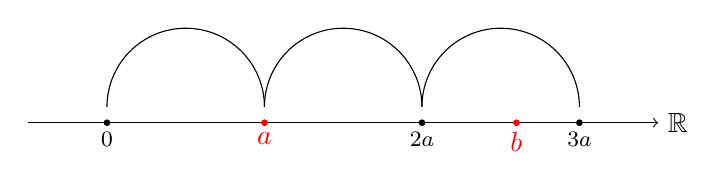
\begin{tikzpicture}
% Draw the real line
  \draw[->] (-1,0) -- (7,0) node[right] {$\mathbb{R}$};
  
  % Draw the point 'x' and '0'
   \filldraw (0,0) circle (1pt) node[below] {\footnotesize$0$};
  \filldraw[red] (2,0) circle (1pt) node[below] {$a$};
    \filldraw (4,0) circle (1pt) node[below] {\footnotesize $2a$};
        \filldraw (6,0) circle (1pt) node[below] {\footnotesize$3a$};
  \filldraw[red] (5.2,0) circle (1pt) node[below] {$b$};

  
 
\draw (2,0.2) arc (0:180:1);
\draw (4,0.2) arc (0:180:1);
\draw (6,0.2) arc (0:180:1);
  
  
  \end{tikzpicture}
\end{document}